% !TEX TS-program = pdflatex
% !TEX encoding = UTF-8 Unicode

% This is a simple template for a LaTeX document using the "article" class.
% See "book", "report", "letter" for other types of document.

\documentclass[11pt]{article} % use larger type; default would be 10pt

\usepackage[utf8]{inputenc} % set input encoding (not needed with XeLaTeX)

%%% Examples of Article customizations
% These packages are optional, depending whether you want the features they provide.
% See the LaTeX Companion or other references for full information.

%%% PAGE DIMENSIONS
\usepackage{geometry} % to change the page dimensions
\geometry{a4paper} % or letterpaper (US) or a5paper or....
% \geometry{margin=2in} % for example, change the margins to 2 inches all round
% \geometry{landscape} % set up the page for landscape
%   read geometry.pdf for detailed page layout information

\usepackage{graphicx} % support the \includegraphics command and options
\usepackage{float} 


% \usepackage[parfill]{parskip} % Activate to begin paragraphs with an empty line rather than an indent

%%% PACKAGES
\usepackage{booktabs} % for much better looking tables
\usepackage{array} % for better arrays (eg matrices) in maths
%\usepackage{paralist} % very flexible & customisable lists (eg. enumerate/itemize, etc.)
\usepackage{verbatim} % adds environment for commenting out blocks of text & for better verbatim
\usepackage{subfig} % make it possible to include more than one captioned figure/table in a single float
% These packages are all incorporated in the memoir class to one degree or another...

%%% HEADERS & FOOTERS
\usepackage{fancyhdr} % This should be set AFTER setting up the page geometry
\pagestyle{fancy} % options: empty , plain , fancy
\renewcommand{\headrulewidth}{0pt} % customise the layout...
\lhead{}\chead{}\rhead{}
\lfoot{}\cfoot{\thepage}\rfoot{}

%%% SECTION TITLE APPEARANCE
\usepackage{sectsty}
\allsectionsfont{\sffamily\mdseries\upshape} % (See the fntguide.pdf for font help)
% (This matches ConTeXt defaults)

%%% ToC (table of contents) APPEARANCE
\usepackage[nottoc,notlof,notlot]{tocbibind} % Put the bibliography in the ToC
\usepackage[titles,subfigure]{tocloft} % Alter the style of the Table of Contents
\renewcommand{\cftsecfont}{\rmfamily\mdseries\upshape}
\renewcommand{\cftsecpagefont}{\rmfamily\mdseries\upshape} % No bold!

%%% END Article customizations

\usepackage[spanish]{babel}
\usepackage{listings} 
%%% The "real" document content comes below...

\title{Investigación de Lenguajes - LIPS}
\author{Rodrigo Castro\\Jorge Vergara\\Oswaldo Bayona}
%\date{} % Activate to display a given date or no date (if empty),
         % otherwise the current date is printed 

\begin{document}
\maketitle
%\tableofcontents % No hace falta un TOC en un artículo corto

\section{Introducción}

Es una familia de lenguajes que soporta la aplicación de varios estilos de programación 
(multiparadigma) aunque prevalece la programación funcional completamente declarativa.\\

El término programación declarativa se refiere al uso de sentencias con las cuáles se modela el
problema pero no se especifica cómo resolverlo,  el computador es el encargado de encontrar 
la solución utilizando inferencias matemáticas y lógicas, en contraste con la programación
imperativa que requiere que el programador implemente la  solución del problema mediante
algoritmos.\\

\section{Características}


Se lo utiliza principalmente para estudios de la Inteligencia Artificial (AI), porque en ésta área
se requiere que las maquinas razonen usando lógicas formales y varios símbolos, y esa es la especialidad de LISP
ya que fue modelada de forma matemática.\\


Las expresiones matemáticas o en general utilizan notación pre-fix por ejemplo:\\
\\ (4 + (5 / 7))  se expresa + 4 / (5  7)\\
\\ Se pueden declarar funciones y organizarlas en módulos, siguiendo el siguiente esquema:\\
	(defun nombreDeLaFuncion (arg1, arg2, …,argn)”Comentarios” (  Cuerpo ) )\\
	
Es muy sencillo y elegante, la implementación de programas recursivos es mucho más fácil que en el lenguaje C.\\

Todas las variables son punteros, una característica representativa de LISP es que las variables 
no existen como en otros lenguajes, aquí se llaman valores, representa los valores ubicándolos 
en zonas específicas de la memoria (dependiendo de la ubicación se simbolizan los valores
de cadenas y números), conceptualmente se considera que existen todas las representaciones
numéricas y de cadenas en las zonas de la memoria.\\

La memoria se constituye de dos partes: el diccionario de símbolos y la memoria de datos. \\
Es interpretado, aunque en muy pocas versiones también es compilado.\\
Sus tipos de datos átomos son: símbolos,  strings, enteros, reales, racionales, par; y los tipos de
datos compuestos son las Listas; los símbolos se refieren a nombres; en LISP las cadenas de
caracteres son tipos de dato primitivos; los pares o conses (cons cell) es un tipo de dato
atómico que se usa para estructurar otros datos primitivos en forma de pares, incluso se 
pueden agrupar otros pares y estructurar arboles binarios, su esquema es el siguiente 
(car . cdr), donde “car” es el primer átomo del par y “cdr” el segundo átomo; por otra parte una 
Lista es una estructura que se basa también en pares siendo más completa pero sencilla de entender. \\

La memoria utiliza el mecanismo de recolección de basura, si un dato ya no es referenciado es
llevado al recolector. \\
Algunas versiones de LISP son: Emacs Lisp, Common Lisp, Scheme.\\



\section{Historia}
La historia del lenguaje LISP es muy extensa, he aquí un resumen; fue concebido originalmente en 1958 por  
John McCarthy y sus colaboradores en el Instituto Tecnológico de Massachusetts como parte de su labor científica, 
la inteligencia artificial, es el segundo lenguaje de alto nivel seguido de FORTRAN, ambos siguen usándose. \\

LISP (LISt Processing) fue el primer lenguaje desarrollado para estudiar la inteligencia
artificial, lo nuevo que introdujo este lenguaje como aporte a la historia fueron las estructuras
de datos de árbol, el compilador auto-contenido, tipos dinámicos etc.\\



En los años 70 la capacidad tecnológica en cuanto a hardware no estaba tan avanzada razón
por la cual no era viable programar con LISP, haciendo de este lenguaje no tan popular y 
limitando su uso solo para inteligencia artificial en máquinas especialmente diseñadas
llamadas maquinas Lisp, posteriormente quedaron obsoletas entonces la popularidad de Lisp tuvo
un incremento porque ahora era factible la programación de  propósito general. \\

A lo largo de los años fueron apareciendo nuevos dialectos de LISP, entre los cuales podemos
mencionar a InterLISP, Franz Lisp,  ZetaLisp; debido a esta gran variedad, entre los años 1980 y 
1990 se creó un nuevo dialecto compatible con los anteriores llamado Common Lisp, otro 
dialecto muby importante es Scheme escrito por G. Steele y G. Sussman  en 1970.\\


	
\section{Tutorial de Instalación}
Un interprete que podemos utilizar para programar en Lisp es DrRacket. Su instalacion es muy sencilla y rapida.
El entorno de trabajo para programar en este lenguaje se puede apreciar en la Figura 5

\begin{figure}[H]
 \begin{center}
    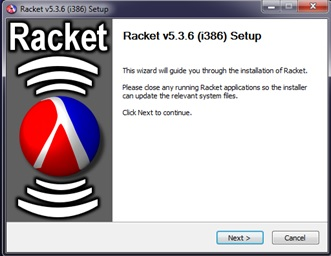
\includegraphics{imagenes_investigacion/paso_uno.jpg}
\end{center}
\caption {}
\label{Figura 1}

\begin{center}
  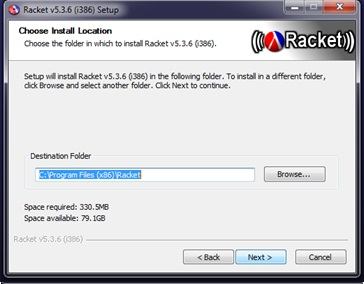
\includegraphics{imagenes_investigacion/paso_dos.jpg}
\end{center}
\caption { }
\label{Figura 2}
\end{figure}


\begin{figure}[H]
   \begin{center}
        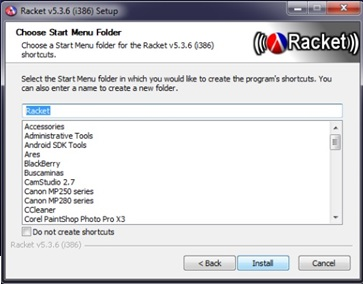
\includegraphics{imagenes_investigacion/paso_tres.jpg}  
   \end{center}
\caption { }
\label{Figura 3}

    \begin{center}
   	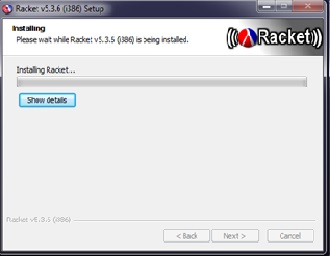
\includegraphics{imagenes_investigacion/paso_cuatro.jpg}
    \end{center}
\caption { }
\label{Figura 4}
\end{figure}


\begin{figure}[H]
\centering
    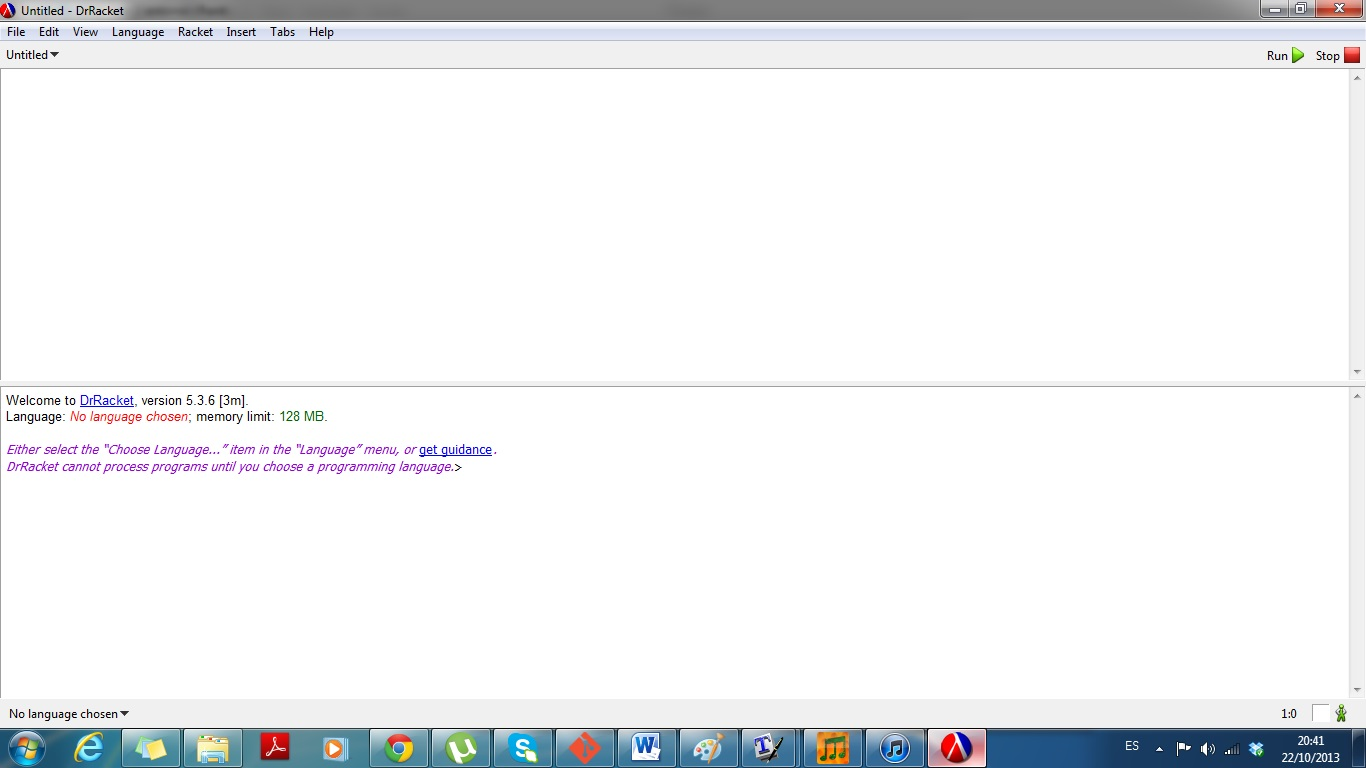
\includegraphics[width=450pts] {imagenes_investigacion/entorno.jpg}
\caption {//Entorno de trabajo de DrRocket}
\label{Figura 5}
\end{figure}



\section{Hola Mundo y otros Programas Introductorios}


%hola mundo
\subsection{Hola Mundo}
\lstset{language=LISP}          

%codigo
\begin{lstlisting}[frame=single] 
	(defun HolaMundo()
		(print 'Hola Mundo')]

\end{lstlisting}

\subsection{Factorial}

% calcular suma de una lista
\lstset{language=LISP}          % Set your language (you can change the language for each code-block optionally)

%codigo 
\begin{lstlisting}[frame=single]
	
	;Calculo del factorial de un numero
	(defun Factorial(n)
		(cond( ( lessp n 2) 1)
			(t  (* n  (Factorial(sub 1 n))] 
\end{lstlisting}

Como se puede ver la funcion factorial tiene una estructura recursiva, adiferencia de los lenguajes de pogramacion tradificionales que tienen sentencias especializadas para realizar iteraciones en LIP no contamos con esas herramientas.\\
Descripcion de la funcion:\\
1.- como paso base vemos si el numero ingresado es menor que 2 devolvemos 1\\
2.-si el numero no es menor que 2 este numero lo multipilcamos por el factorial de n-1 \\

\subsection{Calcular Media Aritmetica de una Lista}

Para resolver este problema lo vamos a dividir en 3 funciones mas bacisas
\\  \\
La primera funcion que vamos a desarrolar es "Suma" que calcula la sumatoria de cada elemento de la lista
% calcular suma de una lista
\lstset{language=LISP}          % Set your language (you can change the language for each code-block optionally)

%codigo 
\begin{lstlisting}[frame=single]
	
	;Suma todos los elementos de una lista
	(defun Suma(lista)
		(cond((null lista) 0 )
			((atom lista) lista)
			(t  (+ (car lista) (suma (cdr lista))] 
\end{lstlisting}

Detallando un poco la funcion:\\
1.- en el caso que la lista este vacia nuestra funcion devuelve 0 nuestro primer caso base\\
2.- si nuestra lista es un atomo es decir un simple numero devolvemos la lista este seria otro caso base\\
3.- en el caso que la lista aun tenga mas de 1 elemento tomamos el 1 elemento de la lista y lo sumamos al resto de elementos de la lista\\

Como segunda parte desarrolarremos una funcion que cuente la cantidad de elementos que se encuentran en la lista

% contar elementos de la lista
\lstset{language=LISP}          % Set your language (you can change the language for each code-block optionally)

%codigo 
\begin{lstlisting}[frame=single]
	
	;cuenta los elementos de la lista
	(defun Contar(lista)
		(cond((null lista) 0 )
			((atom lista) 1)
			(t (addl (contar (cdr lista)] 
\end{lstlisting}

Para completar la solucion al problema implementaremos la ultima funcion que es una especie de funcion principal que pide numeros para una lista y pesenta el valor de la media aritmetica

% calcular media aritmetica
\lstset{language=LISP}          % Set your language (you can change the language for each code-block optionally)

%codigo 
\begin{lstlisting}[frame=single]
	(defun Media() ;calcula la media aritmetica de una lista
		(print 'introdusca la lista')
		(setq lista (read))
		(setq n (contar lista))
		(setq media (/ (sumar lista) n))
		(princ 'la media es = ' ' )
		(print media)]
\end{lstlisting}

Esta funcion es mucha mas sencialla que las 2 anteriores lo unico que hacemos es pedir al usuario que introdusca una lista contamos cuantos elementos tiene con la funcion contar definida anteriormete, calculamos el valor de la suma de los elementos de la lista con la funcion suma, calculamos la media y la presentamos

\section{Bibliografía}


http://www.davidam.com/docu/lisp/lisp2.pdf
http://www.ii.uam.es/~fdiez/docencia/material/lisp0.pdf
http://paulgraham.es/ensayos/lo-que-hizo-diferente-a-lisp.html
http://es.wikipedia.org/wiki/Lisp
http://es.wikibooks.org/wiki/Programaci%C3%B3n_en_LISP
  


\end{document}
